\subsection*{\Large Общая характеристика работы}
\fontsize{14pt}{15pt}\selectfont
\underline{\textbf{Актуальность темы.}} Ленточные конвейеры являются неотъемлемой составляющей транспортных систем горных предприятий в России и за рубежом.
Сложности и особенности динамики движения ленты конвейера, возникающие при переключениях скоростей, пуске и~останове, проскальзывание ленты, особенности случайного грузопотока, зависимость эффективности работы ленточного конвейера от горнотехнических условий, значительный расход электроэнергии при неполной загрузке и работе вхолостую приводят к поиску решения задач оптимизации и автоматизации процессов работы конвейерных установок, к повышению общей эффективности эксплуатации этих сложных систем. В настоящее время системы управления работой ленточных конвейеров на горных предприятиях решают ограниченный круг задач повышения эффективности работы и увеличения срока службы оборудования, и~в~большинстве своем реализуют такие функции, как оперативно-диспетчерское управление (пуск, останов, переключение скорости движения ленты), поддержание определенного уровня производительности, сигнализацию и контроль состояния оборудования.

Таким образом, разработка и техническая реализация новых решений в области автоматизации и управления ленточными конвейерными установками горных предприятий с целью повышения эффективности их эксплуатации является в настоящее время актуальной задачей.
\bigskip

\underline{\textbf{Целью работы}} является разработка новых решений для автоматизации управления и повышения эффективности эксплуатации конвейерного транспорта горных предприятий. В работе получен новый алгоритм останова конвейера, разработана структура и вариант реализации комплексной автоматической системы управления магистральным ленточным конвейером, реализующей алгоритмы, которые позволяют существенно снизить вероятность проскальзывания ленты в исследуемых процессах пуска, останова и изменения скорости движения ленты конвейеров, тем самым повысить эффективность эксплуатации конвейерного транспорта горных предприятий.
\bigskip

\underline{\textbf{Идея работы}} состоит в управляемом регулировании натяжений конвейерной ленты в процессе останова конвейера и разработке комплексной системы автоматического управления ленточным конвейером для повышения эффективности его эксплуатации.
\bigskip

\if 0
\underline{\textbf{Задачи исследования.}} Для~достижения поставленной цели необходимо было решить следующие задачи исследования: 
\begin{enumerate}
	\item модификация реализованной ранее математической модели ленточного конвейера для возможности исследования процессов торможения;
	\item исследование режимов торможения и пуска одноприводного двухбарабанного ленточного конвейера с натяжным устройством, расположенным в хвостовой части;
	\item разработка алгоритмов управления исследуемыми режимами работы конвейера, не допускающих проскальзывание ленты;
	\item разработка структуры комплексной системы автоматического управления, реализующей разработанные алгоритмы;
	\item предложение варианта технической реализации комплексной системы автоматического управления ленточным конвейером.
\end{enumerate}
\bigskip

\fi

\underline{\textbf{Предмет защиты.}} На защиту выносятся следующие основные положения и результаты, обладающие новизной:
\begin{enumerate}
	\item математическая модель ленточного конвейера, дополненная управляющими воздействиями, соответствующими тормозным моментам на барабанах конвейера, которая позволяет учитывать воздействие тормозных устройств при моделировании;
	\item алгоритм управления процессами пуска и останова конвейера, позволяющий осуществлять управляемое торможение хвостового барабана ленточного конвейера, не допуская проскальзывания ленты;
	\item методика выбора и расчета параметров алгоритма управления остановом конвейера позволяет использовать разработанный алгоритм для конвейеров различных модификаций;
	\item структура комплексной автоматической системы управления ленточным конвейером, реализующей следящие алгоритмы пуска, торможения и переключения скорости движения ленты, не допускающие проскальзывания.
\end{enumerate}
\bigskip

\underline{\textbf{Научная новизна работы}} состоит в том, что:
\begin{enumerate}
	\item разработанная математическая модель магистрального ленточного конвейера позволяет моделировать и исследовать процессы пуска и торможения;
	\item разработанные алгоритмы управления позволяют существенно снизить вероятность проскальзывания конвейерной ленты при изменениях скорости ее движения;
	\item разработанная методика расчета параметров робастных алгоритмов управления позволяет применять их для конвейеров различных типов;
	\item разработанная структура системы управления конвейерной установкой, осуществляет комплексное управление процессами пуска и торможения конвейера;
	\item разработано программное и аппаратное обеспечение цифровой системы управления конвейерной установкой.
\end{enumerate}
\bigskip

\underline{\textbf{Методы исследования.}} При решении поставленных в работе задач использовались методы теории волновых процессов в упругих средах, теоретической механики, классической теории автоматического управления, методы статистического анализа и математического моделирования. Применено современное программное обеспечение Matlab R2012b (8.0.0.783), SIMATIC Step 7, PLCSIM v.5.4 для построения моделей, обработки данных и подтверждения результатов.
\bigskip

\underline{\textbf{Обоснованность и достоверность научных положений}} подтверждается корректным применением известных методов математического анализа, результатами исследований теории колебаний упругих систем, теоретической механики, теории автоматического управления, теории регулируемого электропривода и достаточной близостью результатов модельных исследований результатам работы реального технологического процесса, взятым с осциллограмм натурных испытаний и работы в производственных условиях.
\bigskip

\underline{\textbf{Практическая значимость работы.}} Разработанные в диссертации методы и алгоритмы управления могут быть использованы при проектировании новых и совершенствовании действующих систем управления процессами транспортировки грузов на ленточных конвейерах, а также для обучения студентов, повышения квалификации персонала по автоматизации технологических процессов и в научных исследованиях в области автоматизации и управления. Использование реализованных алгоритмов управления в промышленности позволит снизить износ ленты конвейеров, уменьшить расходы электроэнергии, а также минимизировать динамические усилия в ленте, что снизит коэффициент запаса по прочности ленты, позволяя использовать менее дорогие типы ленты и продлить срок ее службы.
\bigskip

\underline{\textbf{Личный вклад автора}} заключается в постановке целей и формулировке задач исследований, доработке существующих математических моделей исследуемого объекта, проведении экспериментов с математическими моделями исследуемого объекта, исследовании и моделировании методов управления процессами пуска и торможения конвейера в различных условиях, разработке и~отладке алгоритмов управления исследуемыми процессами, разработке методики расчета и выбора параметров алгоритмов управления, проведении модельных исследований разработанных алгоритмов управления и анализе их работы, реализации разработанных алгоритмов управления на современном промышленном оборудовании для автоматизации.
\bigskip

\underline{\textbf{Апробация работы.}} Основные положения и результаты диссертационной работы докладывались и обсуждались на научной секции XIV Международной студенческой олимпиады по автоматическому управлению BOAC’2011 (НИУ ИТМО, 2011 г.), на ежегодном научном симпозиуме «Неделя горняка» (МГГУ, 2012, 2014 г.), на Международном форуме-конкурсе молодых ученых «Проблемы недропользования» (НМСУ «Горный», 2014 г.), на научных семинарах кафедры «Автоматика и управление в технических системах» (МГГУ, 2012 -- 2014 гг.).
\bigskip

\underline{\textbf{Публикации.}} По теме диссертации опубликовано 8 научных работ в периодических изданиях и в сборниках научных трудов, в том числе 5 работы в~изданиях, рекомендованных ВАК Минобрнауки.
\bigskip

\underline{\textbf{Объем и структура работы.}} Диссертация состоит из~введения, четырех глав, заключения и~четырех приложений. Полный объем диссертации составляет 126~страниц с~58~иллюстрациями и~9~таблицами. Список литературы содержит 81 наименование.

%\newpage\texttt{}
\subsection*{\Large Содержание работы}

Во \underline{\textbf{введении}} обоснована актуальность проблемы, исследуемой в рамках диссертационной работы, сформулирована цель, изложены основные научные положения, выносимые на защиту, отмечена научная новизна и практическая значимость, указаны сведения об апробации представляемой работы.
\bigskip

\underline{\textbf{Первая глава}} посвящена анализу теоретических и технических решений задач автоматизированного управления ленточными конвейерами для повышения эффективности их эксплуатации. Выполнен анализ основных результатов исследований, посвященных данной теме.

Регулирование скорости движения ленты конвейера, оптимизация пусковых и тормозных процессов, а также контроль проскальзывания ленты позволяет существенно повысить эффективность эксплуатации транспортных машин. Лента является основным и наименее долговечным элементом ленточного конвейера. Ее стоимость может составлять около половины общей стоимости конвейера, а высокие амортизационные затраты на обслуживание ленты -- немаловажный фактор при определении области применения и экономической эффективности конвейерного транспорта. Поэтому оптимизация режимов работы конвейерной установки, направленная на увеличение срока службы ленты, оказывает существенное влияние на общую эффективность эксплуатации ленточных конвейеров.

Основные факторы, которые отрицательно сказываются на сроке службы конвейерной ленты~-- это динамические нагрузки при переключении скорости ее~движения, а также проскальзывание ленты в различных режимах работы конвейера. Проскальзывание ленты на приводном барабане может возникать при~разгоне или торможении конвейера, и это отрицательно влияет не только на~срок службы ленты, но и на срок службы привода конвейера. Этот фактор можно исключить или свести к минимуму, применяя различные способы управления, которые основаны на своевременном изменении натяжений в ветвях конвейера таким образом, чтобы соблюдалось условие Эйлера.

Проблемам разработки алгоритмов оптимизации работы ленточных конвейеров, синтеза регуляторов и систем управления, проведению модельных и~натурных исследований посвящено множество научных работ, разработаны различные структурные схемы систем и алгоритмов регулирования, в том числе оптимальных. В первой главе рассмотрены работы следующих авторов: Дмитриевой В. В., Мамалыги В. М., Петкова О. Н., Сухарева И. А., Сокотнюка Ю. А., Гершуна С. В., Серикова С. А., Черемушкиной М. С., Мартынова В. В., Городецкого А. В., Кангина В. В. Симонса А..

Анализ рассмотренных работ показал, что проблема снижения износа ленты при останове ленточного конвейера не имеет окончательного решения. В~настоящее время, в связи с развитием промышленной микропроцессорной управляющей техники появилась возможность решения этой проблемы современными методами. Это позволило сформулировать следующие задачи исследования в области автоматизации и управления конвейерными установками:
\begin{itemize}
	\item исследование существующей математической модели ленточного конвейера, описанной в работе В. В. Дмитриевой, и ее уточнение для последующих исследований эксплуатации конвейерной установки в режимах пуска и торможения;
	\item исследование переходных процессов пуска и торможения конвейера и поиск способов управления этими процессами с целью оптимизации и повышения эффективности работы конвейера;
	\item разработка и исследование алгоритмов управления, оптимизирующих переходные процессы пуска и торможения конвейера. Эти алгоритмы управления должны обеспечивать номинальные значения натяжений в грузовой и~порожней ветвях конвейера для исключения проскальзывания ленты на~приводном барабане при торможении или свободном выбеге конвейера, а~после его останова исключать провисание ленты между роликоопорами. Это позволит уменьшить износ ленты, что, в свою очередь, позволит сократить расходы на обслуживание и ремонт, продлит срок службы конвейерной установки;
	\item разработка структуры и варианта реализации комплексной системы автоматического управления ленточным конвейером, в которой реализуются алгоритмы управления процессами пуска и торможения конвейера, а также другие алгоритмы управления, повышающие эффективность эксплуатации ленточного конвейера. Эта задача также включает в себя разработку программного обеспечения и подбор аппаратного обеспечения для построения комплексной системы автоматического управления.
\end{itemize}

\underline{\textbf{Вторая глава}} посвящена исследованию пуско-тормозных режимов работы одноприводного двухбарабанного ленточного конвейера с натяжным устройством, расположенным в хвостовой части. В~главе рассматривается выбор и описание математической модели ленточного конвейера, ее доработки, требуемые для дальнейших исследований, а также анализ переходных процессов, возникающих при пуске, изменении скорости и торможении ленточного конвейера. В частности, представлен анализ переходных процессов, возникающих при переключении скорости ленты конвейера, анализ переходных процессов, возникающих при торможении как приводного, так и хвостового барабана конвейера, анализ переходных процессов, возникающих при останове (свободном выбеге) конвейера.

\begin{figure} [h!] 
	\center
	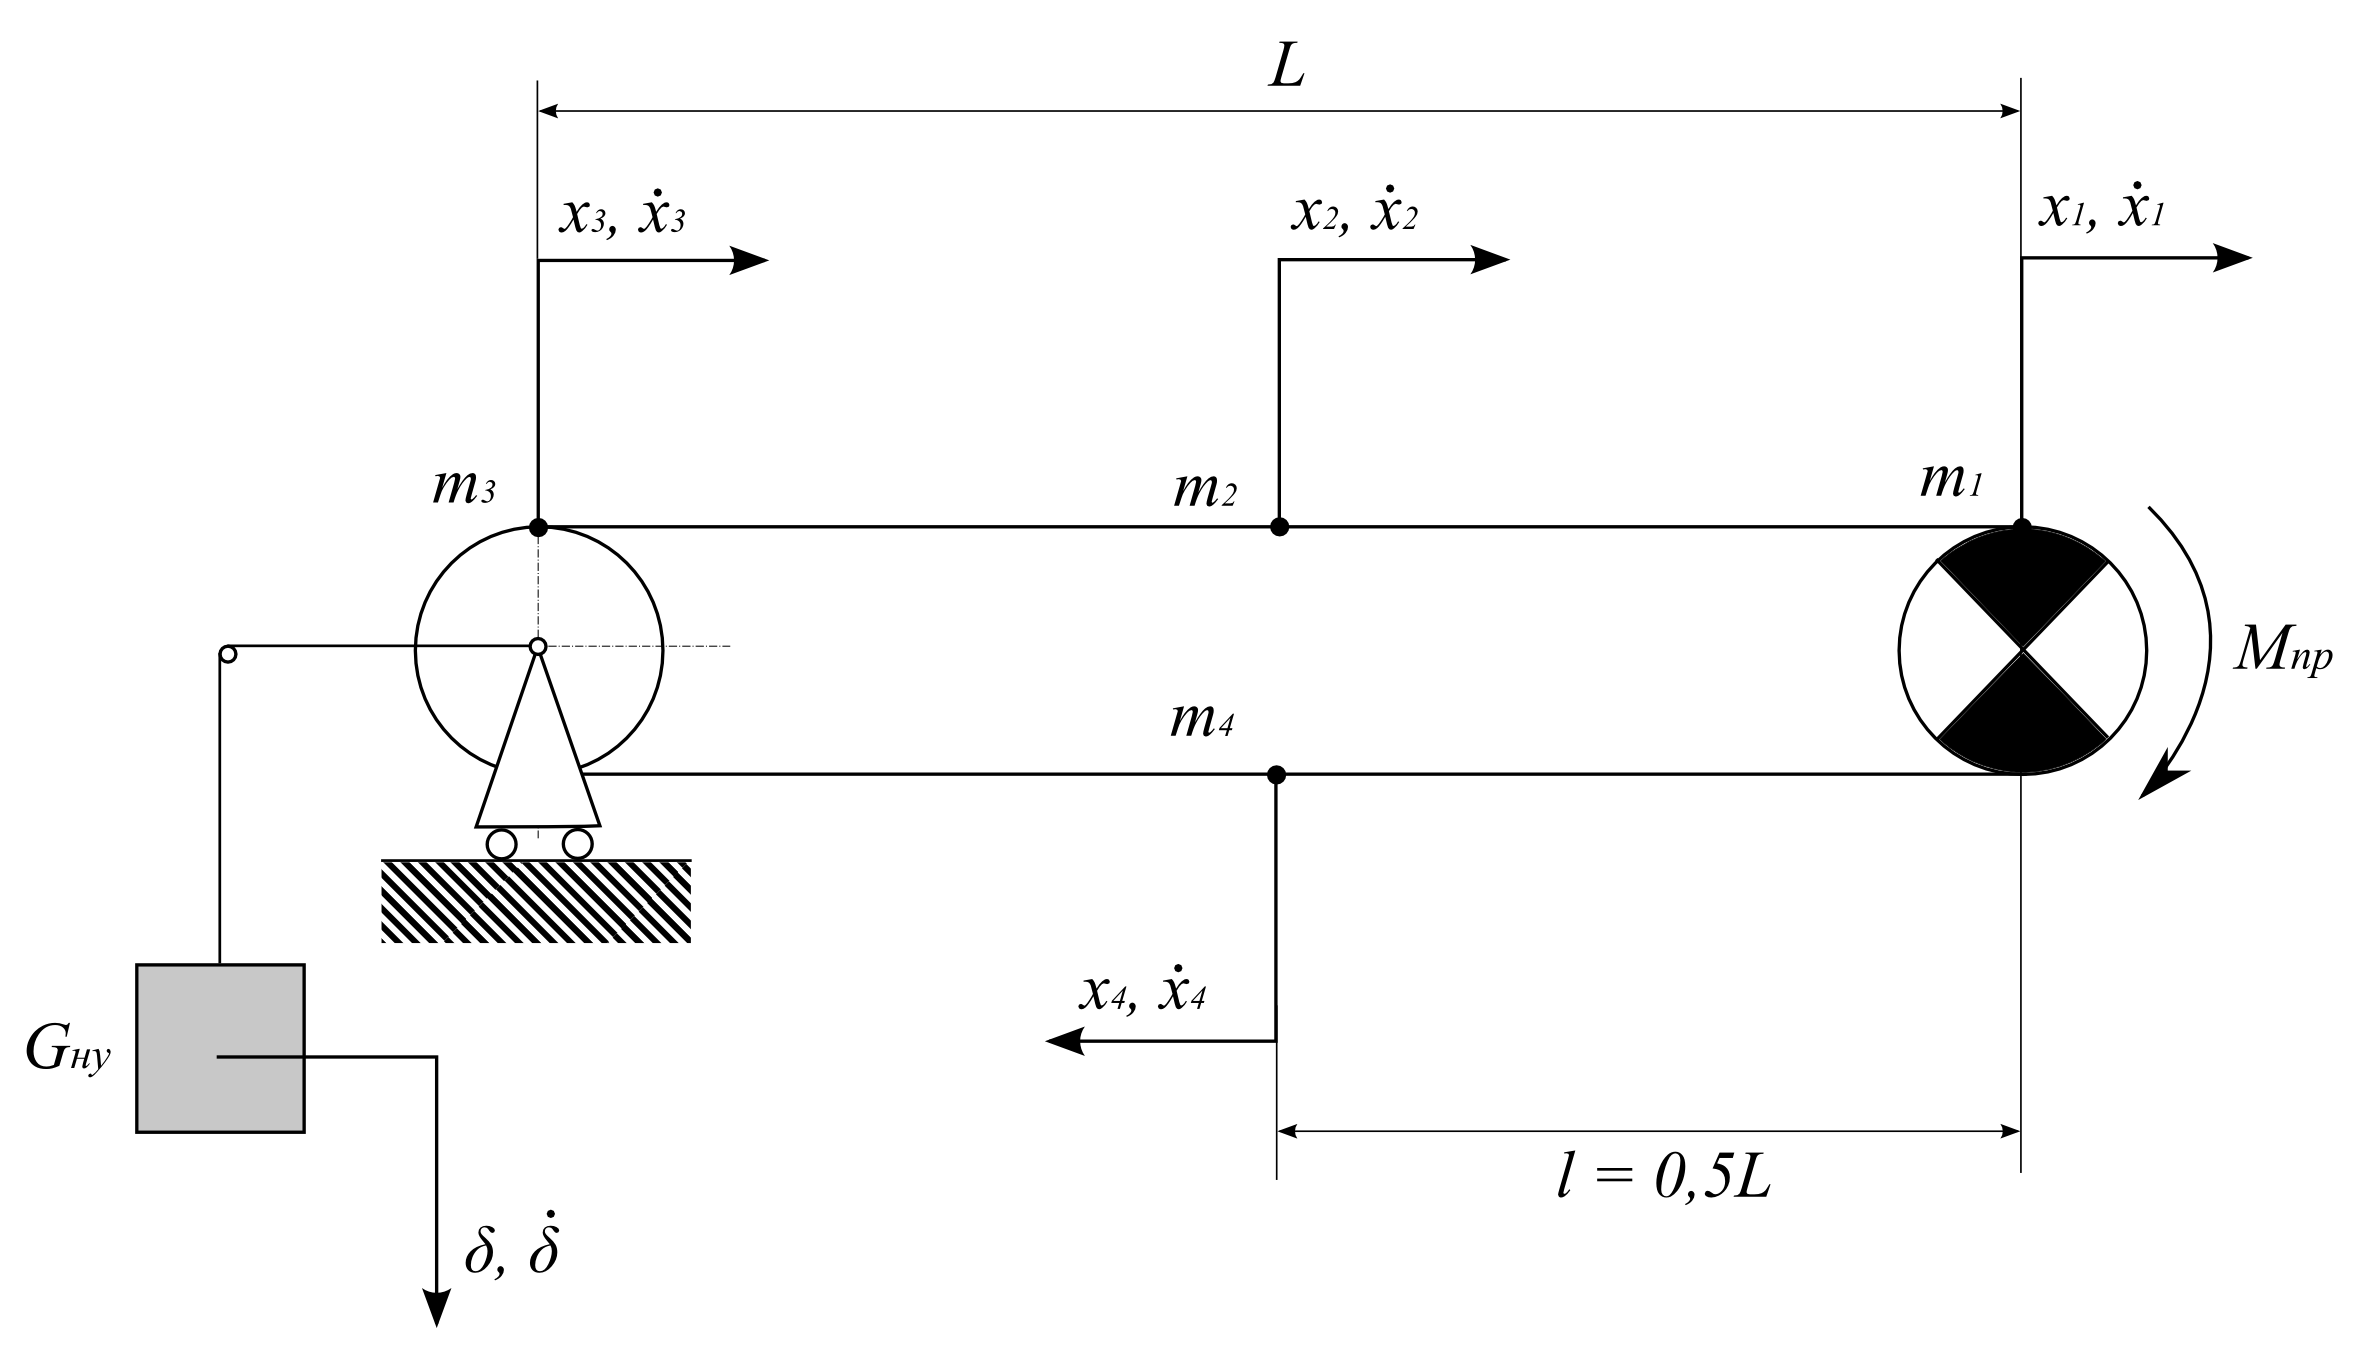
\includegraphics [scale=0.2] {3-1-0}
	\caption{Расчетная схема конвейера с натяжным устройством, расположенным в хвостовой части конвейера.} 
	\label{img:3.sheme}
\end{figure}

Для~исследования выбран подземный ленточный конвейер \textbf{1Л-100К} с~тканевой лентой, предназначенный для~использования в~выработках с~углами наклона от $ -3^\circ $ до $ +18^\circ $. Приемная способность этого конвейера составляет $11\text{м}^3/\text{мин}$, ширина ленты $1000\text{мм}$, скорость движения ленты $1,6\text{м/с}$, диаметр приводного барабана  $800\text{мм}$, производительность  $420\text{т/час}$. Длина конвейерной установки при угле наклона выработки $ 0^\circ $  составляет $1000\text{м}$. Конвейер имеет однобарабанный привод с~тяговым фактором $e^{\mu\alpha} = 2,5$.\\

Описана математическая модель ленточного конвейера, полученная в работе В. В. Дмитриевой, а также произведена ее модификация для возможности управления натяжным и тормозными устройствами. Для этого исходная модель конвейера разделена на две связанных между собой модели: модель, описывающую движение ленты, и модель, описывающую движение натяжного устройства.

В модели движения ленты переменными являются перемещения $ x_1, x_2, x_3, x_4 $, скорости $ \dot x_1, \dot x_2, \dot x_3, \dot x_4 $ и ускорения $ \ddot x_1, \ddot x_2, \ddot x_3, \ddot x_4 $ четырех сосредоточенных масс. Положение и скорость натяжного устройства $ \delta $ и $ \dot \delta $ считаются внешними воздействиями $ U_1 $ и $ U_2 $. В схеме моделирования, реализованной в~Simulink, лента конвейера представлена своей внутренней моделью состояний, построенной на основе системы дифференциальных уравнений, описывающих движение ленты конвейера.

Для модели натяжного устройства переменными являются перемещение груза $ \delta $, скорость его перемещения $ \dot \delta $ и ускорение $ \ddot \delta $. Перемещения сосредоточенных масс $ x_3 $ и $ x_4 $ считаются внешними управляющими воздействиями $ U_3 $ и $ U_4 $. Система уравнений, описывающая динамику натяжного устройства, записывается в следующем виде:
\begin{equation}
\label{eq:nu_model1}
\begin{array}{rcl}
\dot z_1 = z_2,\\ \nonumber
\dot z_2 = - \frac{C_K g}{G_\text{ну}} z_1 + 0.5 \frac{C_K g}{G_\text{ну}} U_3 - 0.5 \frac{C_K g}{G_\text{ну}} U_4 - g - \frac{f}{g} z_2.\\
\end{array}
\end{equation}

где $ U_3 $ -- перемещение сосредоточенной массы, расположенной на~приводном барабане, $ U_4 $ -- перемещение сосредоточенной массы, расположенной на~хвостовом барабане, $ C_k $ -- жесткость канатов натяжного устройства, $ G_{\text{ну}} $ -- вес натяжного устройства, $ g $ -- ускорение свободного падения.

Связь между моделями замкнутого контура ленты и натяжного устройства представлена в~виде структурной схемы на рис.~\ref{img:3.common_struct}.

\begin{figure} [h] 
	\center
	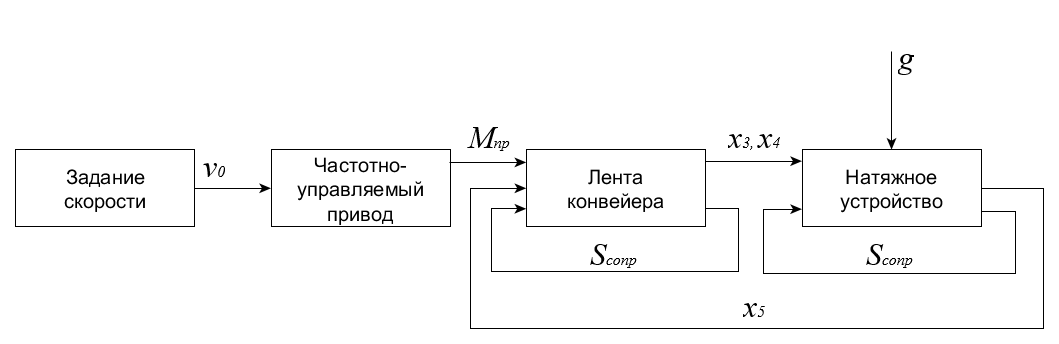
\includegraphics [scale=0.45] {3-6}
	\caption{Структурная схема связи моделей ленты и натяжного устройства, которая обеспечивает возможность управления натяжным устройством} 
	\label{img:3.common_struct}  
\end{figure}

В схеме моделирования, реализованной в Simulink, натяжное устройство представлено своей внешней моделью, построенной на основе системы уравнений, описывающих динамику натяжного устройства (рис. \ref{img:ext}).

\begin{figure} [h!] 
	\center
	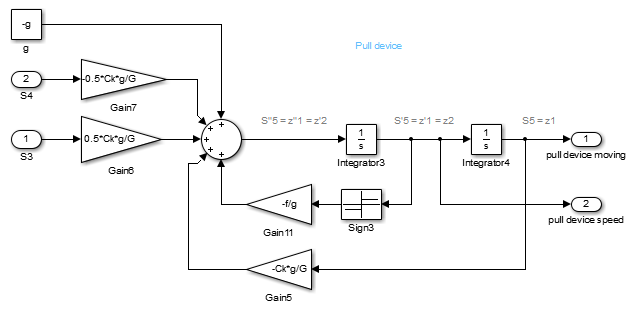
\includegraphics [scale=0.8] {3-7}
	\caption{Структурная схема модели натяжного устройства} 
	\label{img:ext}  
\end{figure}

Для возможности исследования процессов торможения была проведена дальнейшая модификация математической модели. При задействовании тормозного устройства на валу барабана возникает дополнительный (тормозной) момент $ M_T $, действующий противоположно направлению движения барабана конвейера. В случае двухбарабанного конвейера имеется возможность прикладывать тормозное усилие к приводному барабану и к хвостовому барабану, поэтому рассматриваются два тормозных момента $ M_{T \text{пр}} $ и $ M_{T \text{хв}} $ соответственно.

В общей модели конвейера тормозные моменты можно рассматривать как~дополнительные управляющие воздействия для модели движения ленты. Тогда система дифференциальных уравнений модифицированной модели конвейера с~учетом этого принимает следующий вид:
$$ \dot X = \tilde AX + \tilde B_\text{пр}U + \tilde B_\text{ну}U_\text{ну} + \tilde B_s U_s +  \tilde{B_{T \text{пр}}} U_{T \text{пр}} +  \tilde{B_{T \text{хв}}} U_{T \text{хв}}, $$

где $ U_{T \text{пр}} = M_{T \text{пр}}$ -- тормозной момент на приводном барабане,  $ U_{T \text{хв}} = M_{T \text{хв}} $ -- тормозной момент на хвостовом барабане.

В работе приводится расчет матриц расширенной модели конвейера, учитывающей тормозные моменты как дополнительные управляющие воздействия.

Компьютерное моделирование режимов работы конвейера производилось в системе Simulink, входящей в пакет прикладных программ Matlab. Проведено исследование следующих режимов работы ленточного конвейера:
\begin{enumerate}
	\item Пуск конвейера и переключение с меньшей скорости на большую;
	\item Останов конвейера без использования торможения (свободный выбег);
	\item Останов конвейера с использованием торможения приводного барабана;
	\item Торможение хвостового барабана конвейера.
\end{enumerate}

Анализ переходных процессов рассмотрен как для режимов пуска и разгона, так и для режима останова (торможения) конвейера. На основе проведенного анализа определен набор алгоритмов управления и функций, которые должны входить в состав разрабатываемой комплексной автоматической системы управления конвейером. Проведенный анализ также позволил сформулировать требования и рекомендации к разрабатываемым алгоритмам и комплексной автоматической системе управления конвейером.
\bigskip

\underline{\textbf{Третья глава}} описывает разработку и исследование работы алгоритмов управления процессами останова и пуска конвейера, которые включают в себя стабилизацию тягового фактора для устранения проскальзывания ленты при торможении конвейера и контроль провисания ленты в грузовой ветви конвейера после его останова.

Разработан алгоритм управления остановом, основанный на предварительном торможении хвостового барабана по определенному закону для управляемого изменения натяжений ленты в точках набегания на приводной барабан и сбегания с приводного барабана. 

Исследован алгоритм управления пуском, который представляет собой последовательность действий, осуществляющую пуск конвейера в условиях измененных при торможении значений натяжений ленты в ветвях конвейера с~целью уменьшения нагрузки на привод во время пуска.
\bigskip

Общий принцип работы алгоритма управления остановом состоит в том, чтобы при инициировании останова конвейера осуществить торможение хвостового барабана таким образом, чтобы возникающие при этом динамические натяжения в ветвях конвейера изменили значение тягового фактора $ \frac{1}{e^{\mu\alpha}} $ до такой величины, при которой с момента отключения привода до момента останова приводного барабана проскальзывание ленты на нем будет отсутствовать. Отключение привода необходимо осуществлять после достижения значения тягового фактора определенной величины, то есть сигнал на останов привода формируется через некоторое время после инициирования останова конвейера, определяемое скоростью распространения упругих волн в конвейерной ленте.

При разработке алгоритма останова рассмотрен процесс торможения, а~также исследованы изменения натяжений ленты конвейера при торможении хвостового барабана, определена зависимость между динамическими натяжениями ленты и силой трения, возникающей при торможении хвостового барабана. Это позволило осуществлять управляемое изменения тягового фактора непосредственно перед остановом конвейера для обеспечения отсутствия проскальзывания ленты, что и стало основой полученного алгоритма. 

Определена общая методика расчета параметров для работы алгоритма останова конвейера с предварительным торможением хвостового барабана. В~частности, определены зависимости, позволяющие вычислить требуемые значения тормозных моментов для приводного и хвостового барабанов для конвейеров различных модификаций. Для расчета значения тормозного момента, который требуется приложить к хвостовому барабану для стабилизации тягового фактора до величины $ E_0 $, сначала рассчитывается величина динамических натяжений, которые необходимо создать в ветвях конвейера. В работе показано, что справедливо следующее равенство:
$$ E_0 = \frac{S_\text{устП} - W_T}{S_\text{устГР} + W_T}, $$

где $ W_T $ -- величина динамических натяжений, $ {S_\text{устГР}} $ и $ {S_\text{устП}} $ -- значения натяжений в грузовой и порожней ветвях в установившемся режиме соответственно. Тогда величина динамических натяжений, которые необходимо создать в ветвях конвейера, вычисляется по следующей формуле:
$$
\label{eq:4.5.wt}
W_T = \frac{S_\text{устП} - E_0 S_\text{устГР}}{E_0 + 1}.
$$

Величина тормозного момента, который требуется приложить к хвостовому барабану для стабилизации тягового фактора до величины $ E_0 $, рассчитывается по формуле:
$$
\label{eq:4.5.mtail}
M_{\text{Тхв}} = \frac{R(0,5G_{\text{ну}} - (q_{\text{л}} + q_{\text{р}})Lw - S_\text{уП} + W_T)}{2}.
$$

Величина тормозного момента, который требуется приложить к приводному барабану для его блокировки после останова привода, рассчитывается по~формуле:
$$
\label{eq:4.5.mdrive}
% M_\Sigma = M_1 + M_4 = -R_\text{б}(W_{\text{гр}} + W_{\text{п}}) - 4M_{T\text{хв}}.
M_{T \text{пр}} = 4\frac{M_{T\text{хв}}}{R}.
$$

Проведены модельные исследования работы алгоритма останова для конвейера выбранной модификации со значениями тормозных моментов, рассчитанными по приведенным зависимостям. Эти исследования показали, что применение разработанного алгоритма останова конвейера обеспечивает стабилизацию тягового фактора, достаточную для торможения конвейера без проскальзывания ленты. Переходной процесс стабилизации тягового фактора при торможении конвейера представлен на рис. \ref{img:4.ema}.

\begin{figure} [h!] 
	\center
	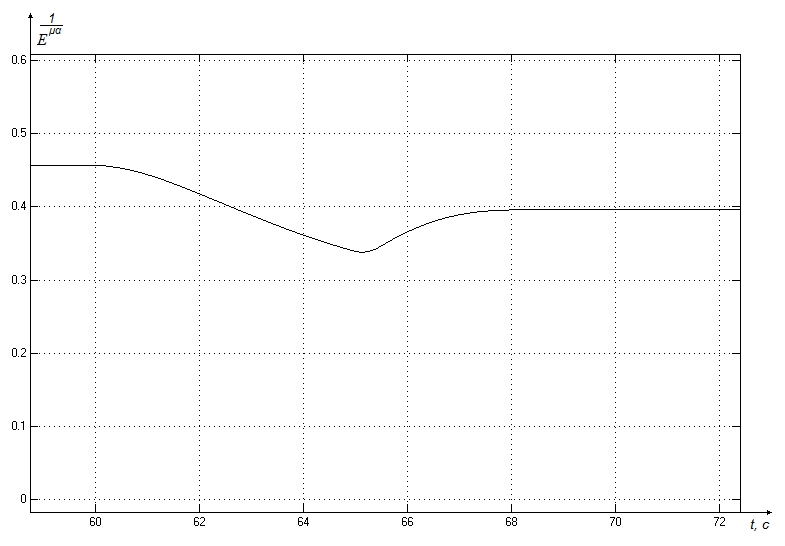
\includegraphics [scale=0.4] {4-11.png}
	\caption{График изменения величины тягового фактора при торможении ленты конвейера с предварительным торможением хвостового барабана, остановом привода и блокировкой приводного барабана после его останова} 
	\label{img:4.ema}  
\end{figure}

Исследованы переходные процессы в ленте конвейера, возникающие при~отключении тормозных устройств после его останова с применением разработанного алгоритма. В рамках исследования было произведено несколько итераций моделирования одновременного отключения тормозных устройств при~различных значениях веса натяжного устройства. Полученные результаты моделирования говорят о том, что отключение тормозных устройств после полного останова конвейера не оказывает негативного эффекта на последующий пуск конвейера и~на~эффективность его работы в целом. Поэтому для пуска конвейера после его остановка с помощью разработанного алгоритма предварительного торможения могут без ограничений использоваться известные алгоритмы.
\bigskip

Проведено экспериментальное исследование работы алгоритма предварительного управляемого торможения конвейера в зависимости от загруженности конвейера. Было проведено моделирование работы алгоритма при различных значениях входящего грузопотока с вычислением требуемого значения тормозного момента. Результаты моделирования показали, что величина тормозного момента, требуемого для корректной стабилизации тягового фактора при минимальном грузопотоке, лишь на 3,16 \% меньше величины тормозного момента, требуемого для корректной стабилизации тягового фактора при максимальном грузопотоке. Если использовать величину тормозного момента хвостового барабана, рассчитанную для максимального значения входящего грузопотока, то~при~случайных изменениях грузопотока изменение величины тягового фактора после стабилизации не превысит 5 \%. Поэтому для любого режима работы конвейера считается допустимым использовать величину тормозного момента, рассчитываемую для максимального значения входящего грузопотока.
\bigskip

В \underline{\textbf{четвертой главе}} приведено описание разработки комплексной автоматической системы управления ленточным конвейером. В~главе рассматривается построение общей структуры комплексной автоматической системы управления конвейерной установкой, включающей в себя различные алгоритмы управления. На основе рассматриваемой структуры системы приводится пример ее реализации с использованием современного программного и аппаратного обеспечения, а также обоснование выбора инструментов для реализации системы и подбор управляющего, исполнительного и измерительного оборудования.

Структура комплексной автоматической системы управления конвейером содержит в себе три подсистемы, каждая из которых реализует определенные алгоритмы управления: подсистему пуска и регулирования скорости (осуществляет запуск конвейера и переключения скорости движения ленты), подсистему стабилизации тягового фактора в номинальном режиме работы (осуществляет управление натяжным устройством таким образом, чтобы величина тягового фактора в номинальном режиме работы не превышала технологического значения для выбранного типа конвейера) и подсистему управления торможением конвейера (осуществляет останов конвейера с использованием алгоритма, предварительного управляемого торможения хвостового барабана). 
\bigskip

Предложен вариант реализации системы управления, который включает в себя предложения по выбору аппаратного обеспечения (программируемых контроллеров, коммуникационных модулей, источников питания), размещению первичных преобразователей для получения информации от объекта управления, а также описывает решение задачи распределенного сбора данных и управления перемещающимися компонентами конвейерной установки. Общая схема варианта реализации системы управления представлена на рис. \ref{img.5.TechR}.
\bigskip

\begin{figure} [h] 
	\center
	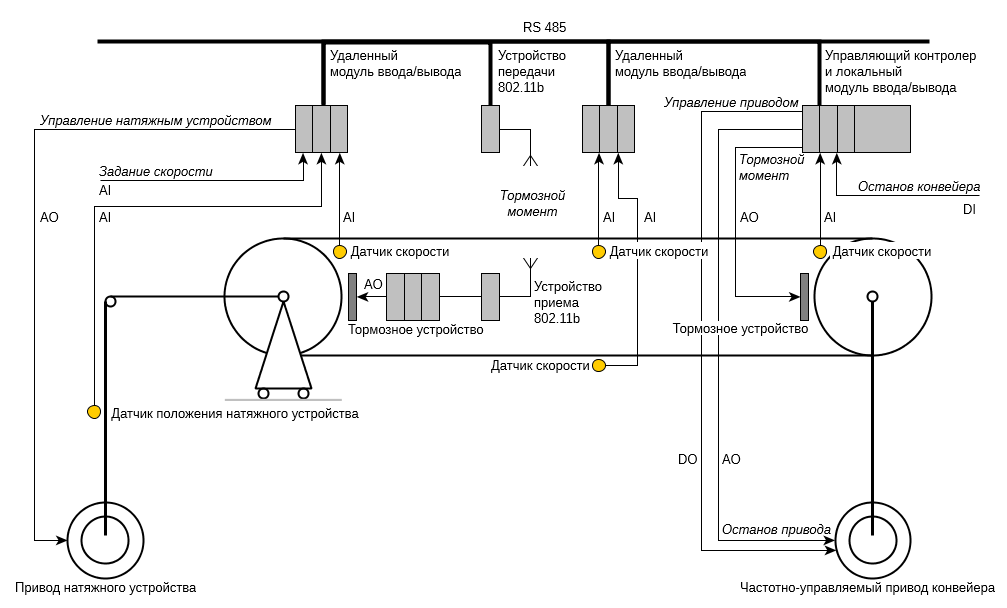
\includegraphics [scale=0.65] {5-4.png}
	\caption{Общая схема технической реализации комплексной системы управления конвейерной установкой} 
	\label{img.5.TechR}  
\end{figure}

В главе также представлены результаты разработки программного обеспечения, реализующего алгоритмы управления системы на промышленном языке программирования стандарта МЭК 61131-3. Исходные коды программ реализации алгоритмов возможно использовать на любом промышленном вычислительном оборудовании, поддерживающем этот стандарт. Это исключает жесткую привязку разработанного программного обеспечения к выбранному оборудованию и позволяет при необходимости построить систему управления с~использованием другого аппаратного обеспечения или использовать разработанное программное обеспечение при построении других автоматических систем управления.
\bigskip

Описаны особенности реализации и отладки комплексной автоматической системы управления конвейерной установкой. Для разработки и отладки алгоритмов управления и технической реализации системы была использована методика компьютерной имитации, в основе которой лежит взаимодействие среды моделирования работы управляющего контроллера и модели конвейерной установки, реализованной в приложении Simulink пакета прикладных программ Matlab, которое позволяет с достаточной степенью детализации и достоверности моделировать не только сам технологический процесс, но и работу технологического оборудования и исполнительных механизмов. Среда моделирования работы управляющего контроллера -- это программное обеспечение, которое обычно разрабатывается производителем управляющего контроллера и позволяет полностью эмулировать его работу, гарантируя идентичность реальным условиям эксплуатации.

В качестве среды моделирования работы управляющего контроллера используется программное обеспечение PLCSIM, входящее в пакет прикладных программ разработки ПО для контроллеров Siemens. PLCSIM позволяет эмулировать работу программируемого контроллера с управляющим  программным обеспечением с возможностью мониторинга состояний сигналов и переменных программы. Общая схема взаимодействия компонентов имитационной среды представлена на рис.~\ref{img.5.imitation1}.

\begin{figure} [h!] 
	\center
	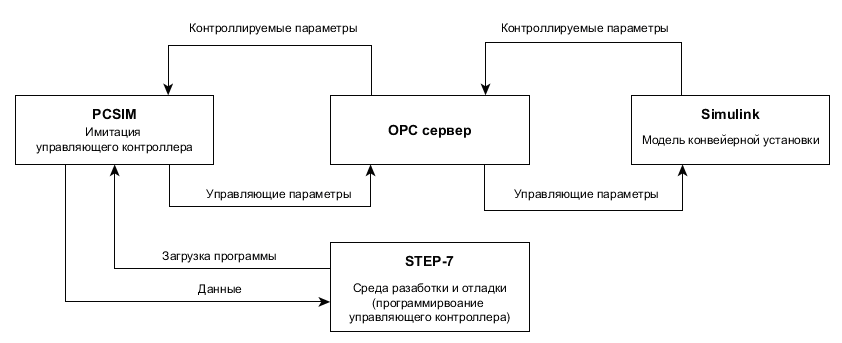
\includegraphics [scale=0.65] {imitation.png}
	\caption{Общая схема взаимодействия компонентов имитационной среды}
	\label{img.5.imitation1}
\end{figure}

Для передачи данных между компонентами имитационной среды был использован OPC-сервер -- программное обеспечение, соответствующее стандарту OPC и предназначенное для совместной работы средств автоматизации. Стандарт ОРС описывает универсальный фиксированный интерфейс обмена данными с~любыми устройствами и программным обеспечением. Программное обеспечение, соответствующее стандарту ОРС, может быть использовано не только для~взаимодействия SCADA-систем с аппаратным обеспечением систем управления, но и для обмена данными между любыми источниками и потребителями данных. Эта возможность была использована при разработке и отладке комплексной системы управления конвейером.
\bigskip

\underline{\textbf{Заключение.}}

В результате проведенных исследований дано новое решение актуальной научно-технической задачи разработки алгоритма предварительного управляемого торможения ленточного конвейера, а также решение задачи реализации алгоритмов автоматического управления ленточным конвейером в виде разработки структуры и варианта реализации комплексной автоматической системы управления ленточным конвейером. Представленные решения позволяют повысить эффективность эксплуатации ленточных конвейеров в различных режимах работы с исключением или минимизацией проскальзывания ленты конвейера на~приводном барабане и существенным снижением динамических усилий в~ленте в~переходных режимах. 

Приведены основные результаты работы, которые заключаются в следующем:
\begin{enumerate}
	\item эффективность эксплуатации конвейерных устройств на горных предприятиях может быть повышена только при условии автоматического управления технологическими операциями, выполняемыми в процессе эксплуатации. Для создания автоматической системы управления конвейерной установкой, позволяющей исключить проскальзывание ленты конвейера на приводном барабане и снизить динамические усилия в ленте в переходных режимах, необходимы управляющие алгоритмы, учитывающие механические свойства  конвейерной ленты и особенности ее поведения: распространение упругих волн, характер возникновения напряжений и деформаций и сил сопротивления движению на различных участках ленты;
	\item произведена модификация существующей математической модели ленточного конвейера. Расширенная математическая модель позволяет исследовать переходные процессы, возникающие при торможении приводного и хвостового барабанов конвейера;
	\item модельные исследования показали, что величина тягового фактора ленточного конвейера при его останове в большинстве случаев превышает технологическое значение, определяемое параметрами конвейера (не соблюдается условие Эйлера), что приводит к проскальзыванию ленты на приводном барабане. На основе модельных исследований был разработан алгоритм управляемого торможения ленточного конвейера, использующий тормозные устройства, расположенные на приводном и на хвостовом барабанах;
	\item разработана методика расчета параметров алгоритма управляемого торможения ленточного конвейера, которая позволяет определить требуемые величины тормозных моментов и тягового фактора, исходя из технологических параметров используемого конвейера;
	\item исследование полученного алгоритма совместно с уточненной математической моделью ленточного конвейера показало, что применение этого алгоритма позволяет минимизировать, а в большинстве случаев исключить проскальзывание ленты при торможении конвейера, а также более чем в~шесть раз сократить временной интервал, в течении которого проскальзывание ленты на приводном барабане гипотетически может возникнуть;
	\item наилучшие результаты повышения эффективности эксплуатации конвейерного транспорта могут быть достигнуты при совместном использовании алгоритмов, осуществляющих не только стабилизацию тягового фактора при торможении конвейера, но и управление другими процессами -- стабилизацией тягового фактора в номинальном режиме работы конвейера и~регулированием скорости движения ленты при переключении для снижения динамических нагрузок. Для этих целей была разработана структура комплексной автоматической системы управления ленточным конвейером, включающая в себя указанные алгоритмы. Предложен вариант реализации системы управления, включающий в себя выбор и обоснование аппаратного обеспечения и компонентов системы, а также разработку программного обеспечения, реализующего управляющие алгоритмы на современном промышленном языке программирования, соответствующем стандарту МЭК 61131-3.
\end{enumerate}

%\newpage
\renewcommand{\refname}{\Large Публикации автора по теме диссертации}
\nocite{*}
\bibliography{biblio}